\section*{圖片}

\begin{figure}[H]  % [H]固定figure於某一頁
\begin{center}
\caption{Trend in Employment and Annual Earnings} \label{emp}
	\begin{subfigure}[b]{0.65\textwidth}
	 	\caption{Employment}\label{emp_e}
		\vspace{-0.85em}
	 	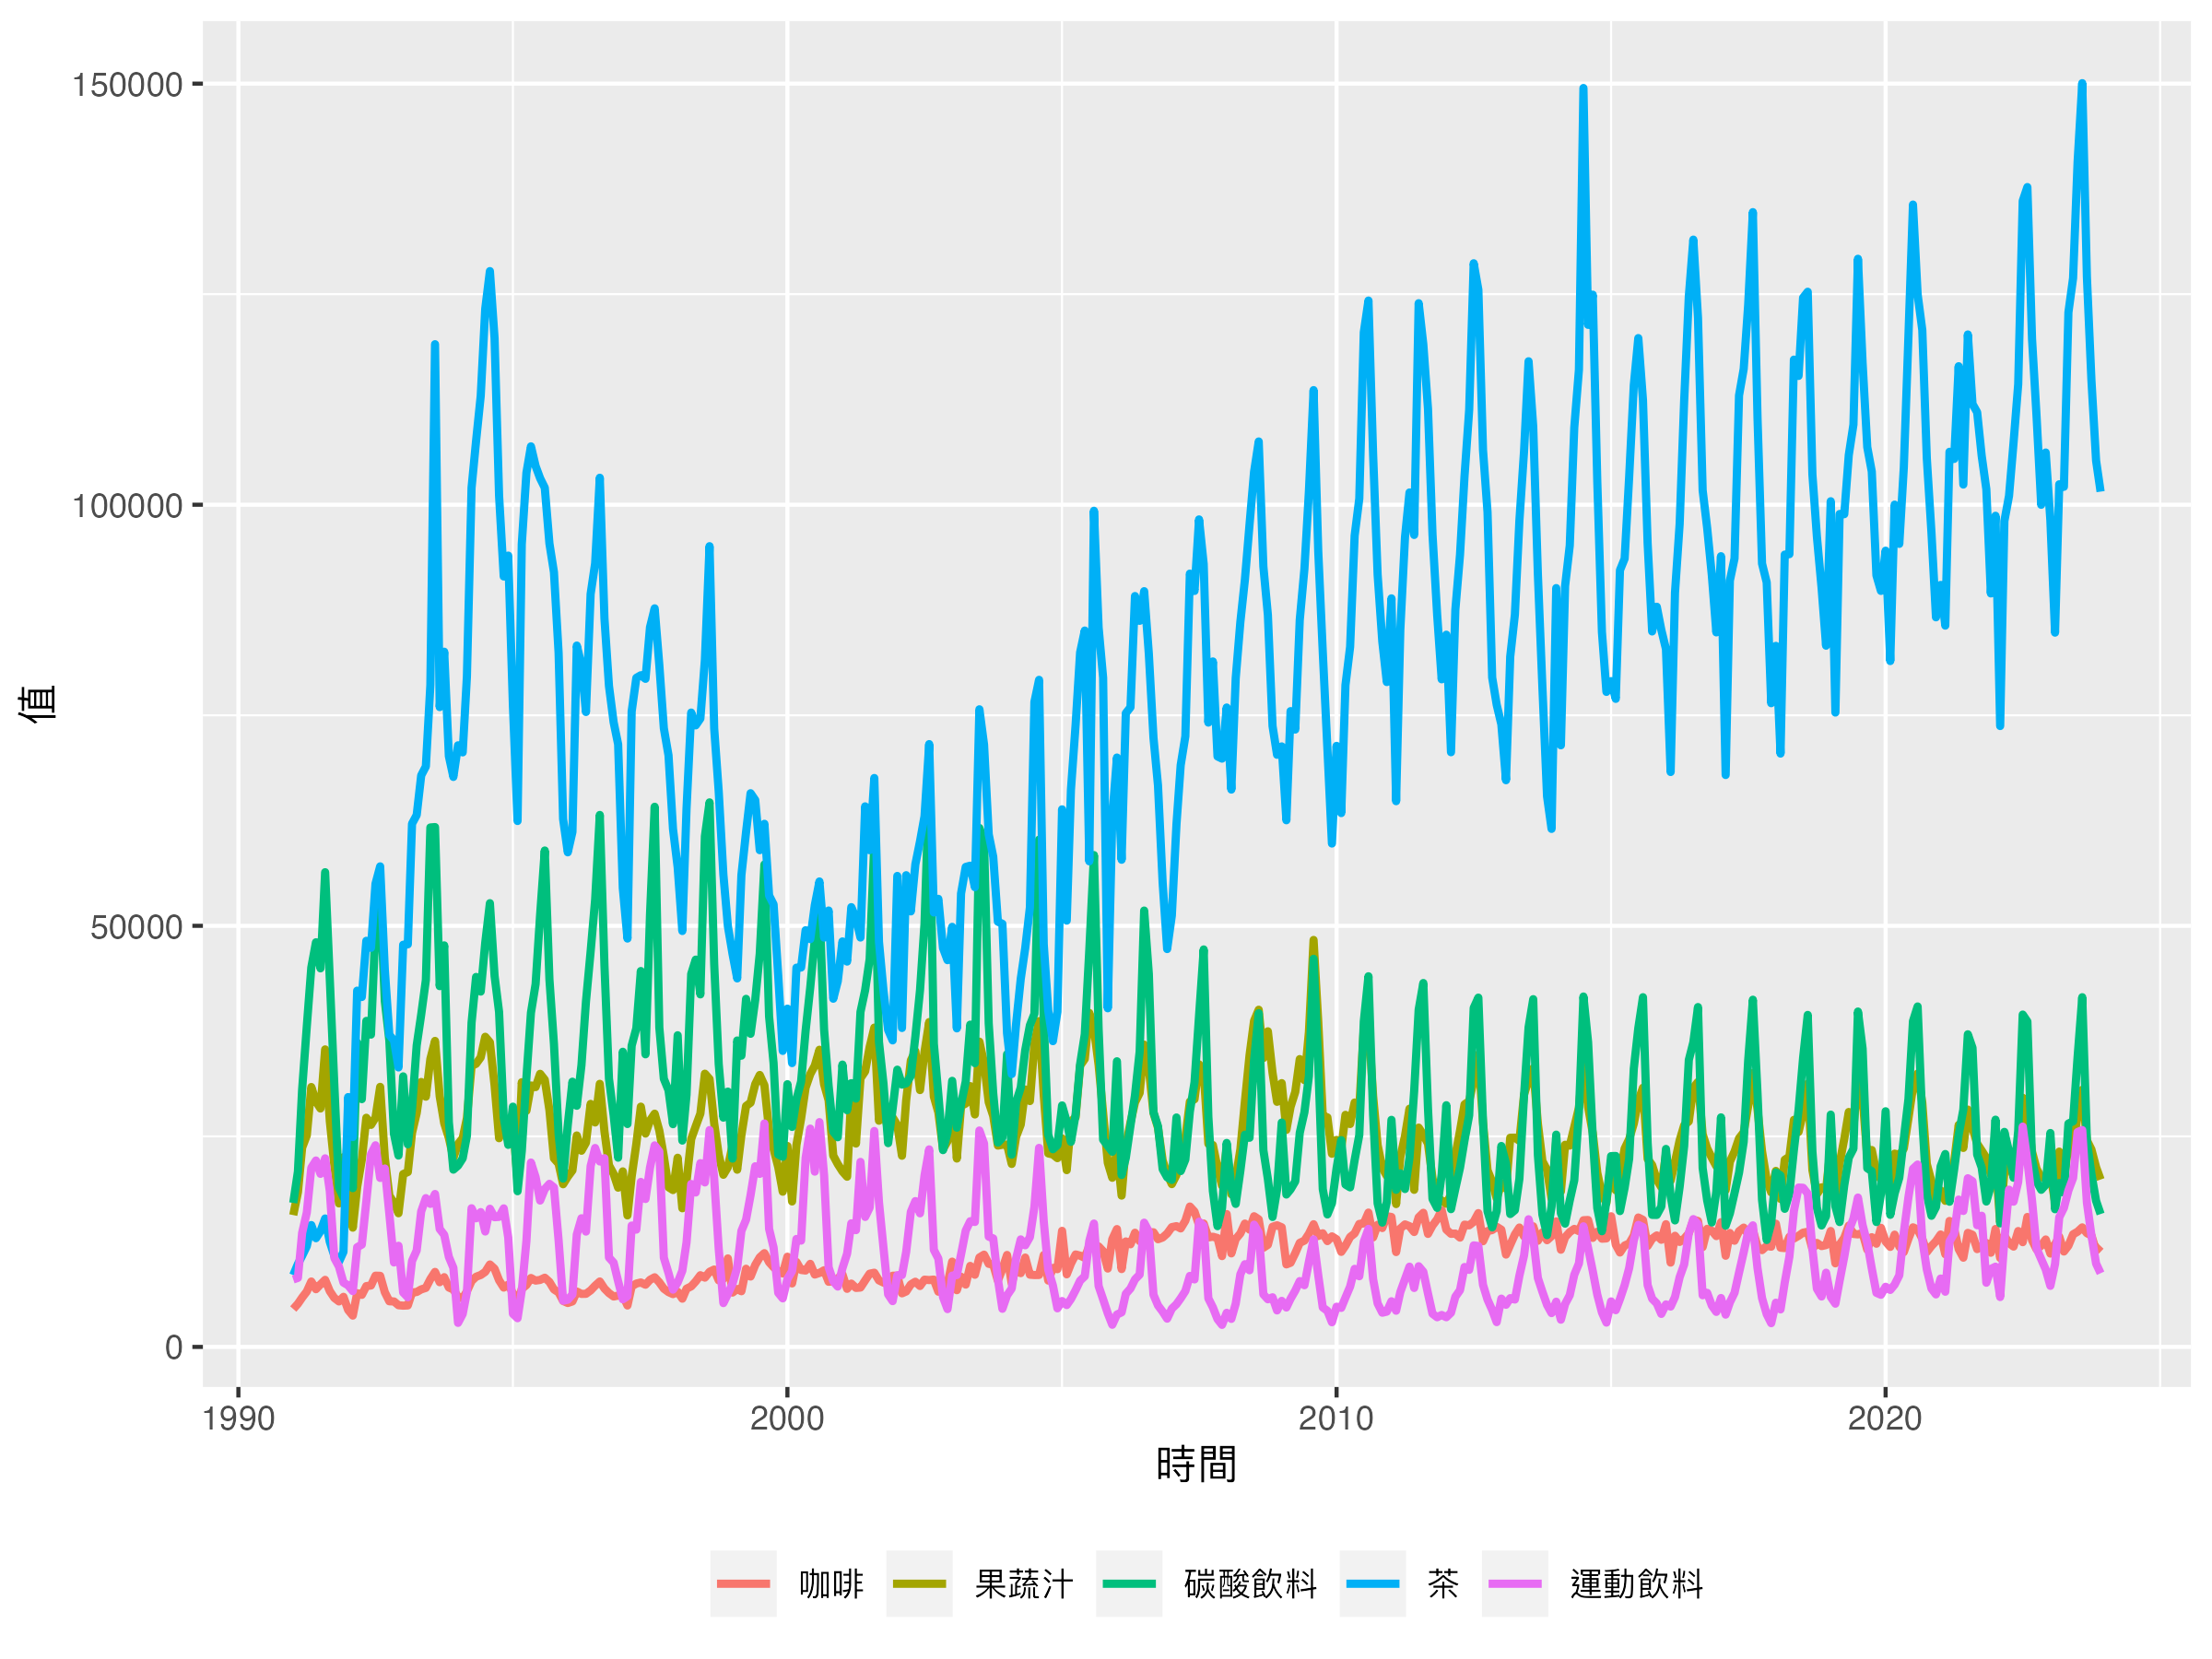
\includegraphics[width=\textwidth]{../outcome/chart1.png}  % both png, jpg can be used for graphs
	 \end{subfigure}
	 \begin{subfigure}[b]{0.65\textwidth}
		\caption{Annual Earnings (1,000 NT\$)} \label{earnings}
		\vspace{-0.85em}
		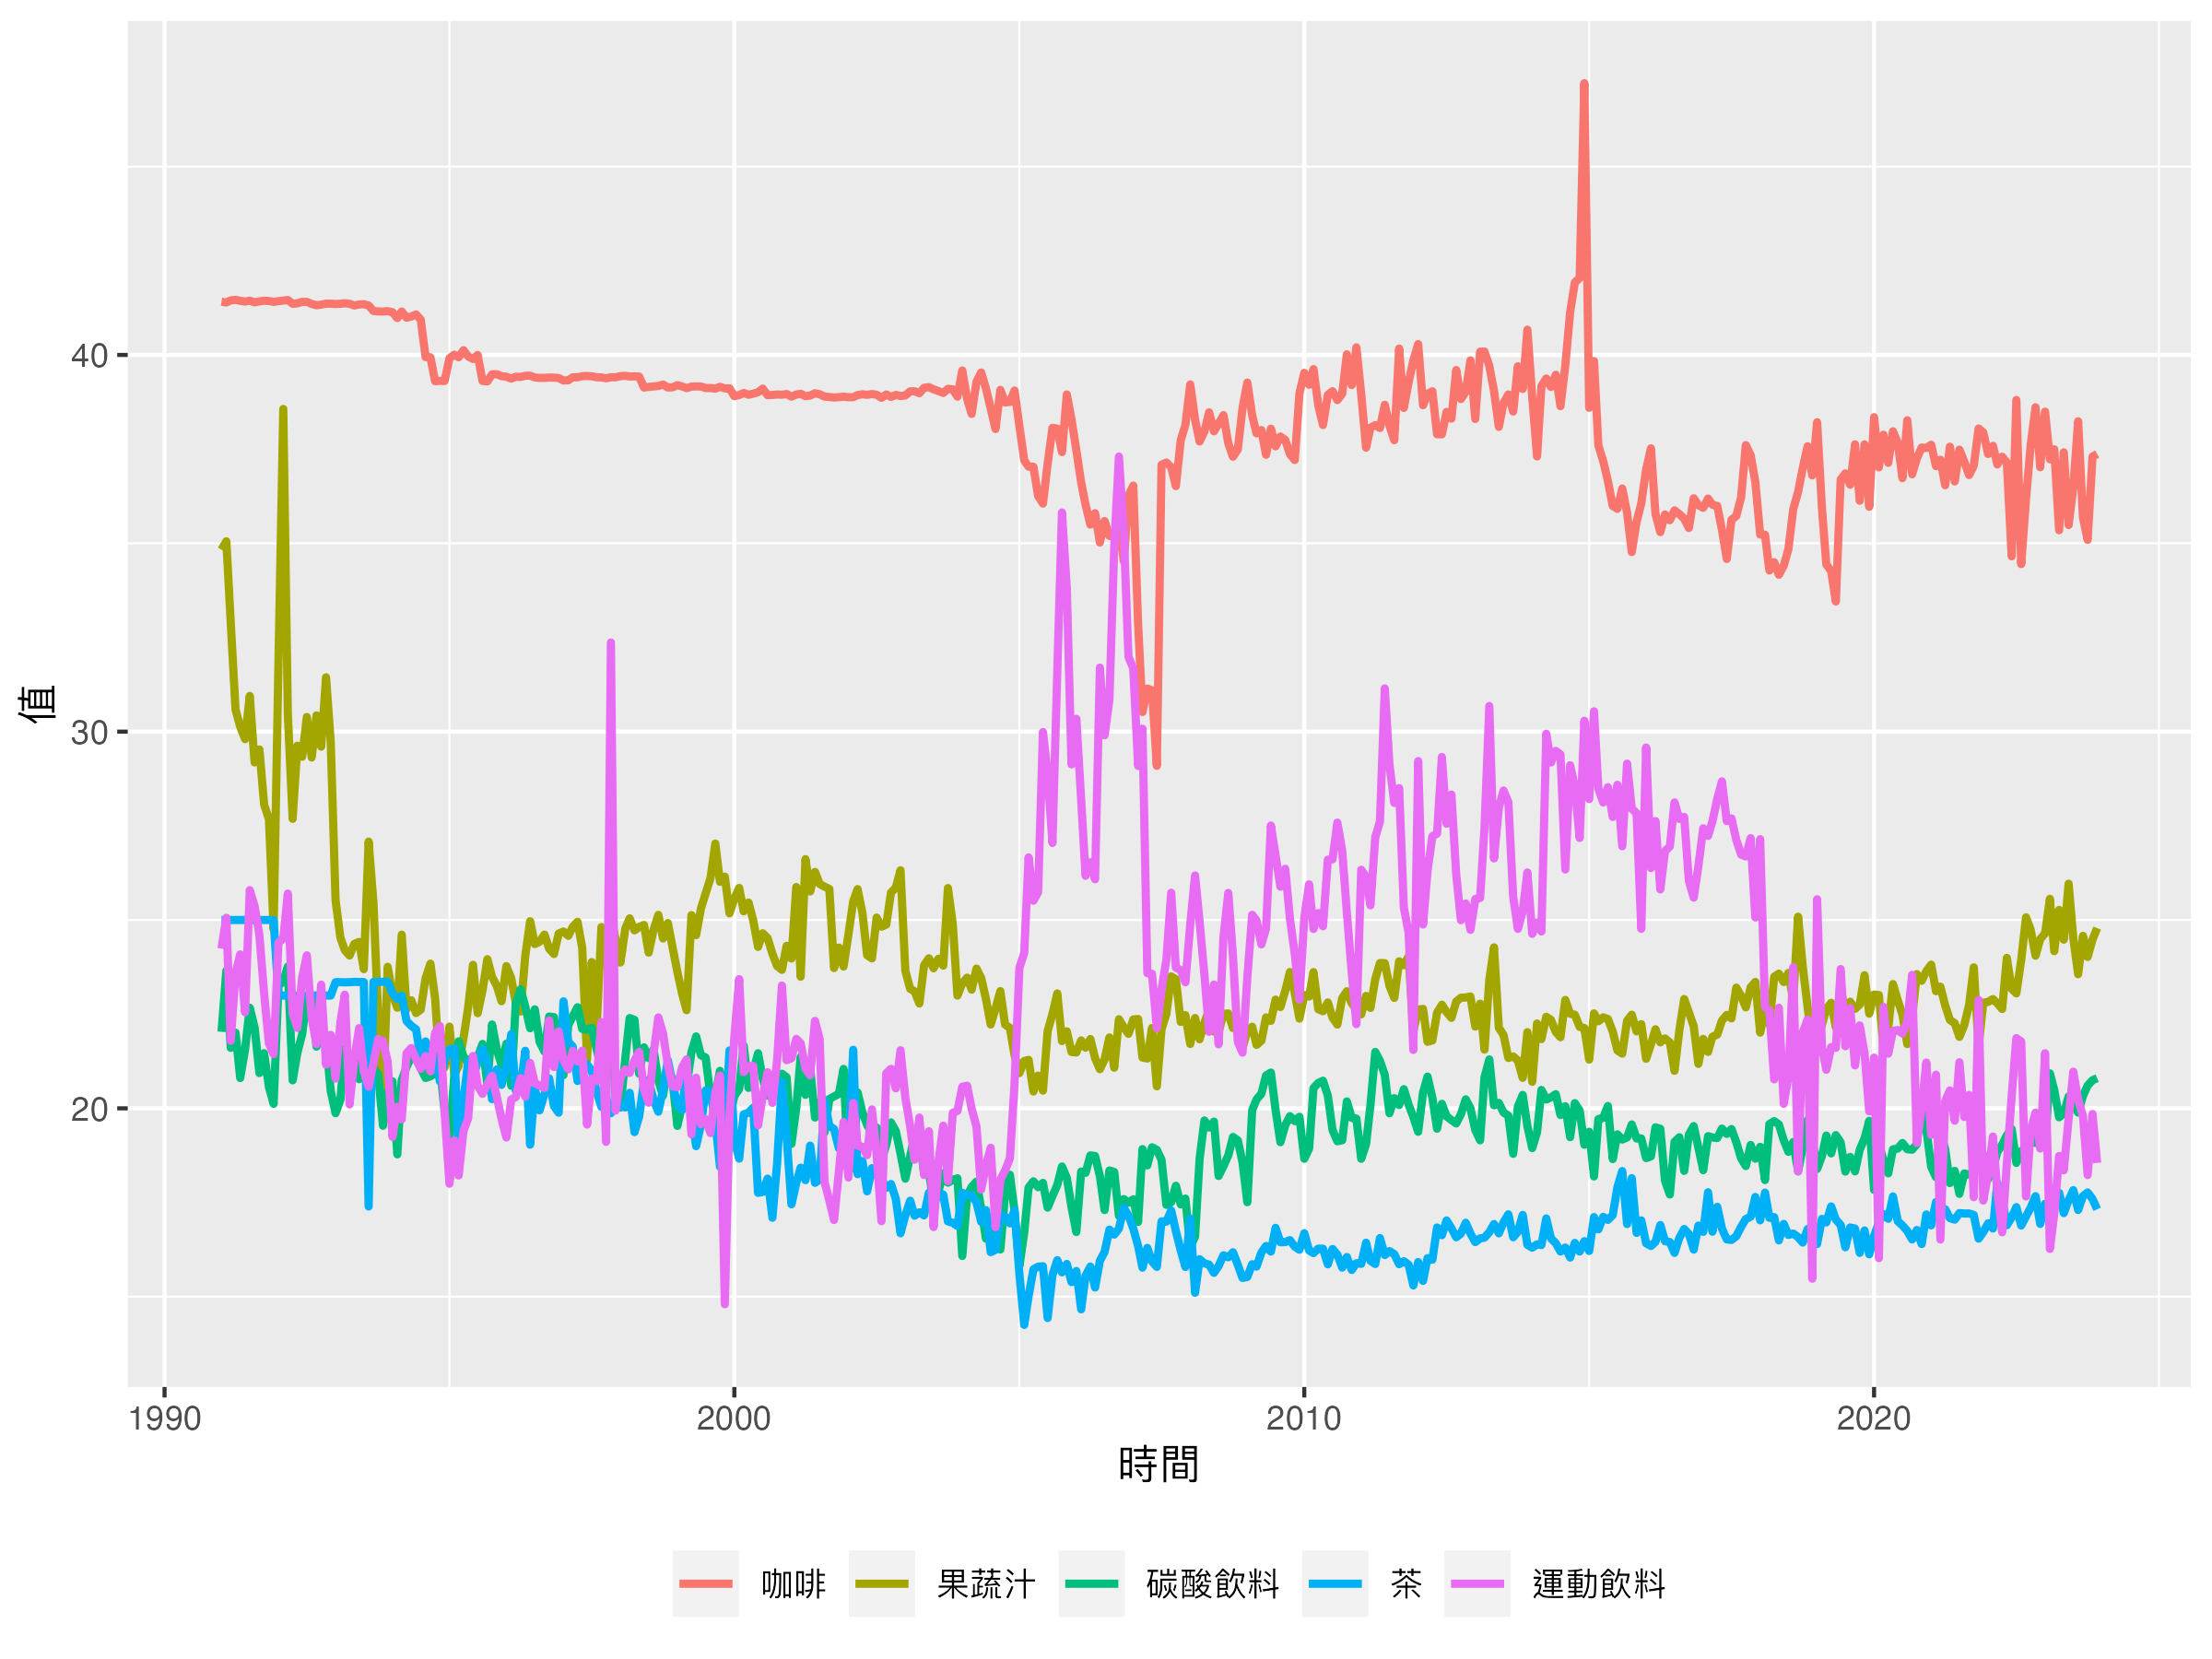
\includegraphics[width=\textwidth]{../outcome/chart2.png}
	\end{subfigure}
\end{center}
\end{figure}
\vspace{-3em}
\begin{singlespace}
        \begin{footnotesize}
        		\noindent {\it Notes:} These figures illustrate the change (from the baseline year) in (a) the proportion of employment (employed at least one month) and (b) annual earnings (NT\$1,000) for the treatment group (i.e., displaced workers) and the comparison group (i.e., non-displaced workers) from five years before to ten years after the (pseudo) displacement year. The vertical axis displays the outcomes at event time $t$ relative to the baseline year ($t = -2$). The horizontal axis refers to the number of years from the (pseudo) displacement year.
        \end{footnotesize}
\end{singlespace}



% \newpage
% \begin{figure}[H]
% 	\centering
% 	\caption{The Relationship Between GDP Per Capita and the Total Fertility Rate}\label{fig.gdp_fertility}
% 	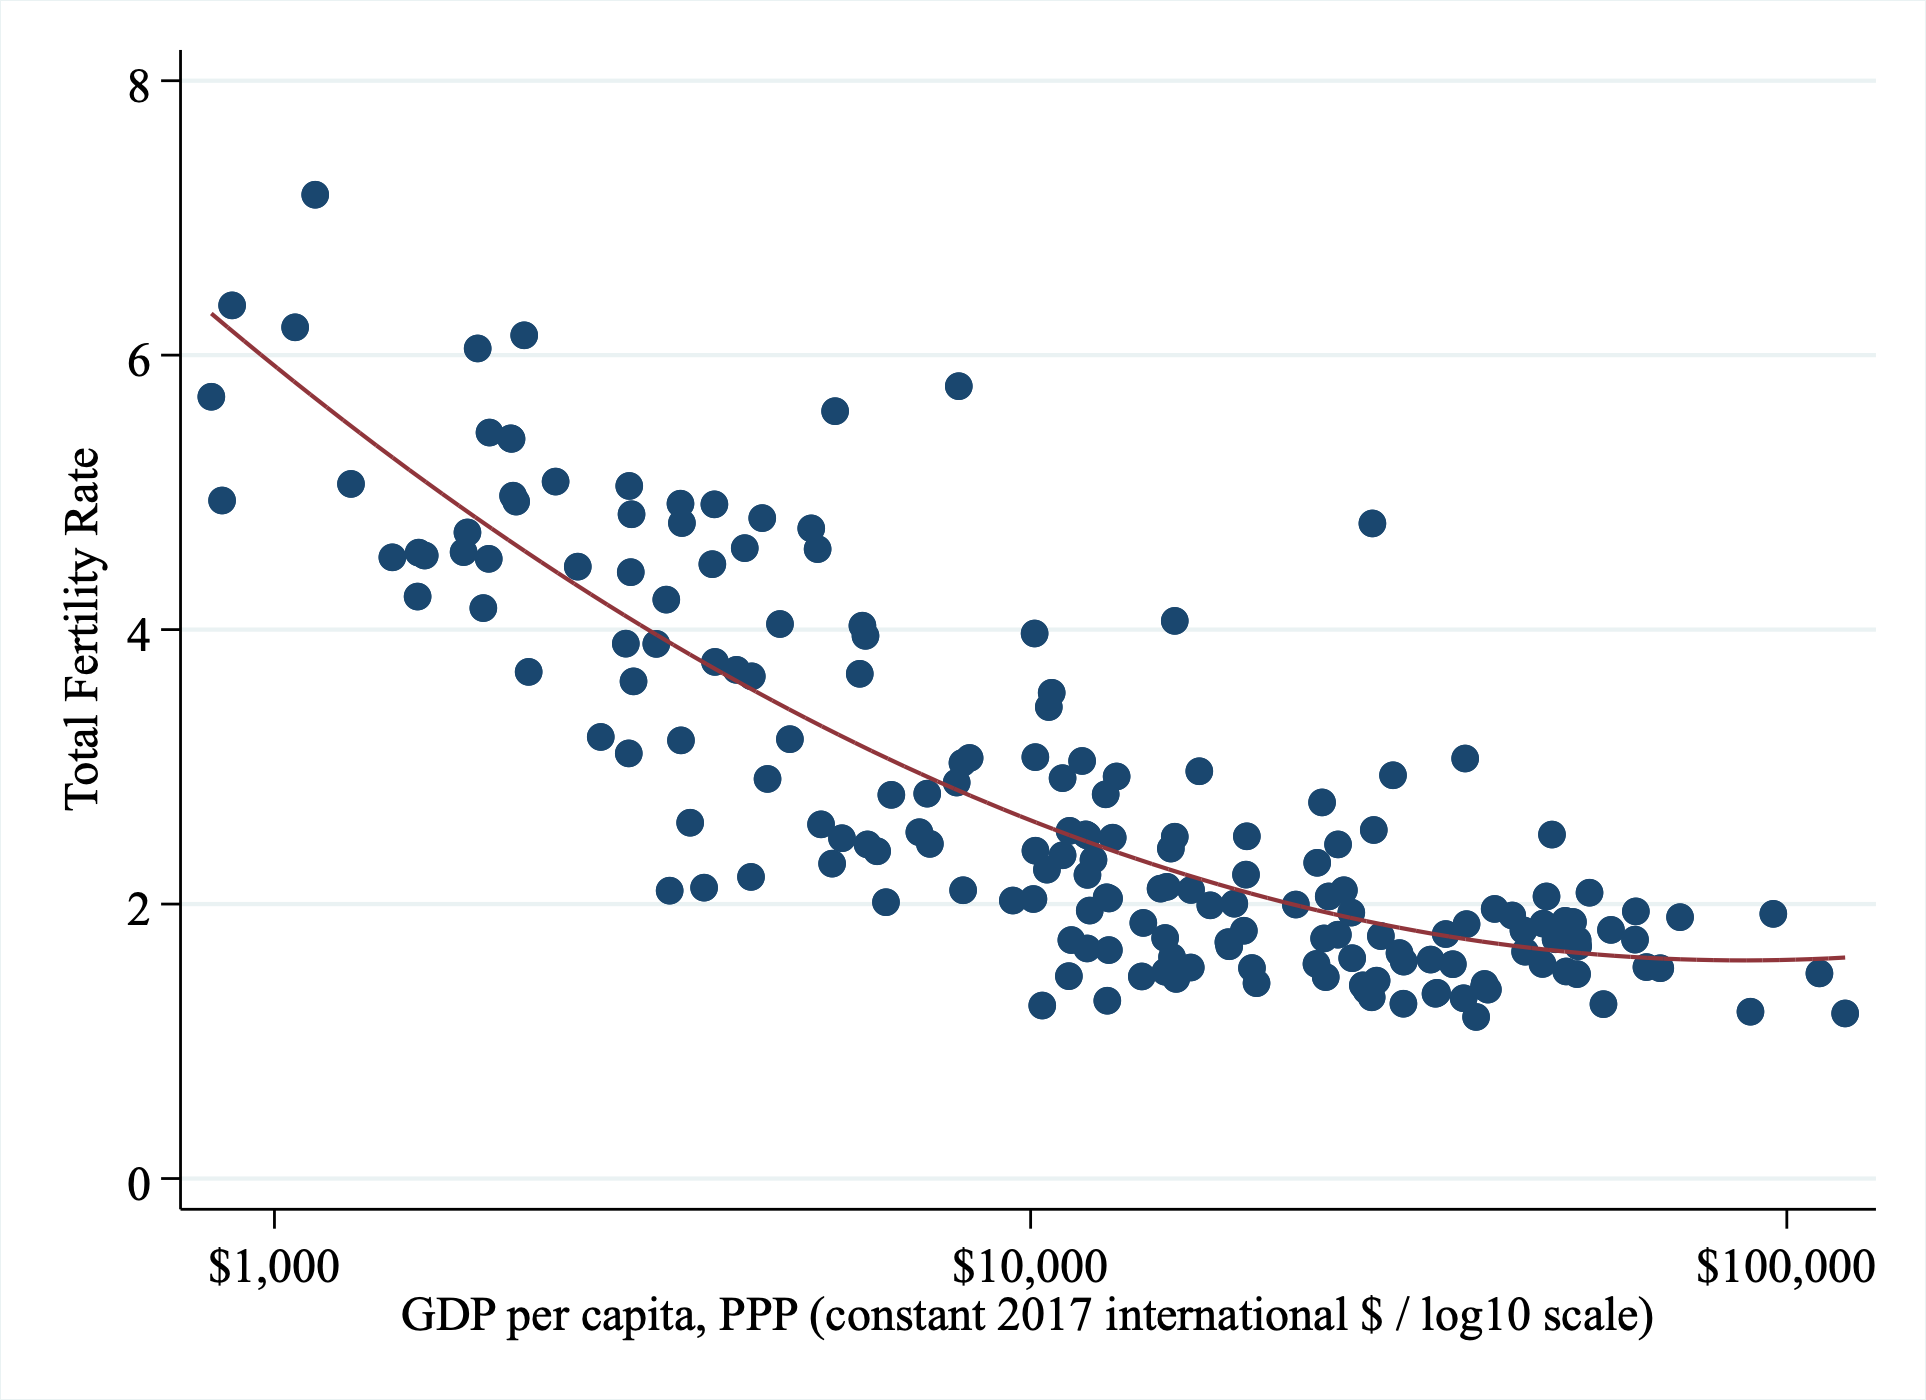
\includegraphics[width=0.8\linewidth]{figures/FC1.jpg}\\
% 	\fontsize{10}{10pt}\selectfont
% 	\flushleft
% 	\emph{Notes:} Each symbol stands for one country. The total fertility rate is defined as the number of children per 1,000 women. The data year is 2020. Data source: Our World in Data \citep{owidfertilityrate,owidgdp}.
% \end{figure}



% \newpage
% \begin{figure}[H]
% 	\centering
% 	\caption{The Relationship Between GDP Per Capita and the Total Fertility Rate}\label{fig.gdp_fertility}
% 	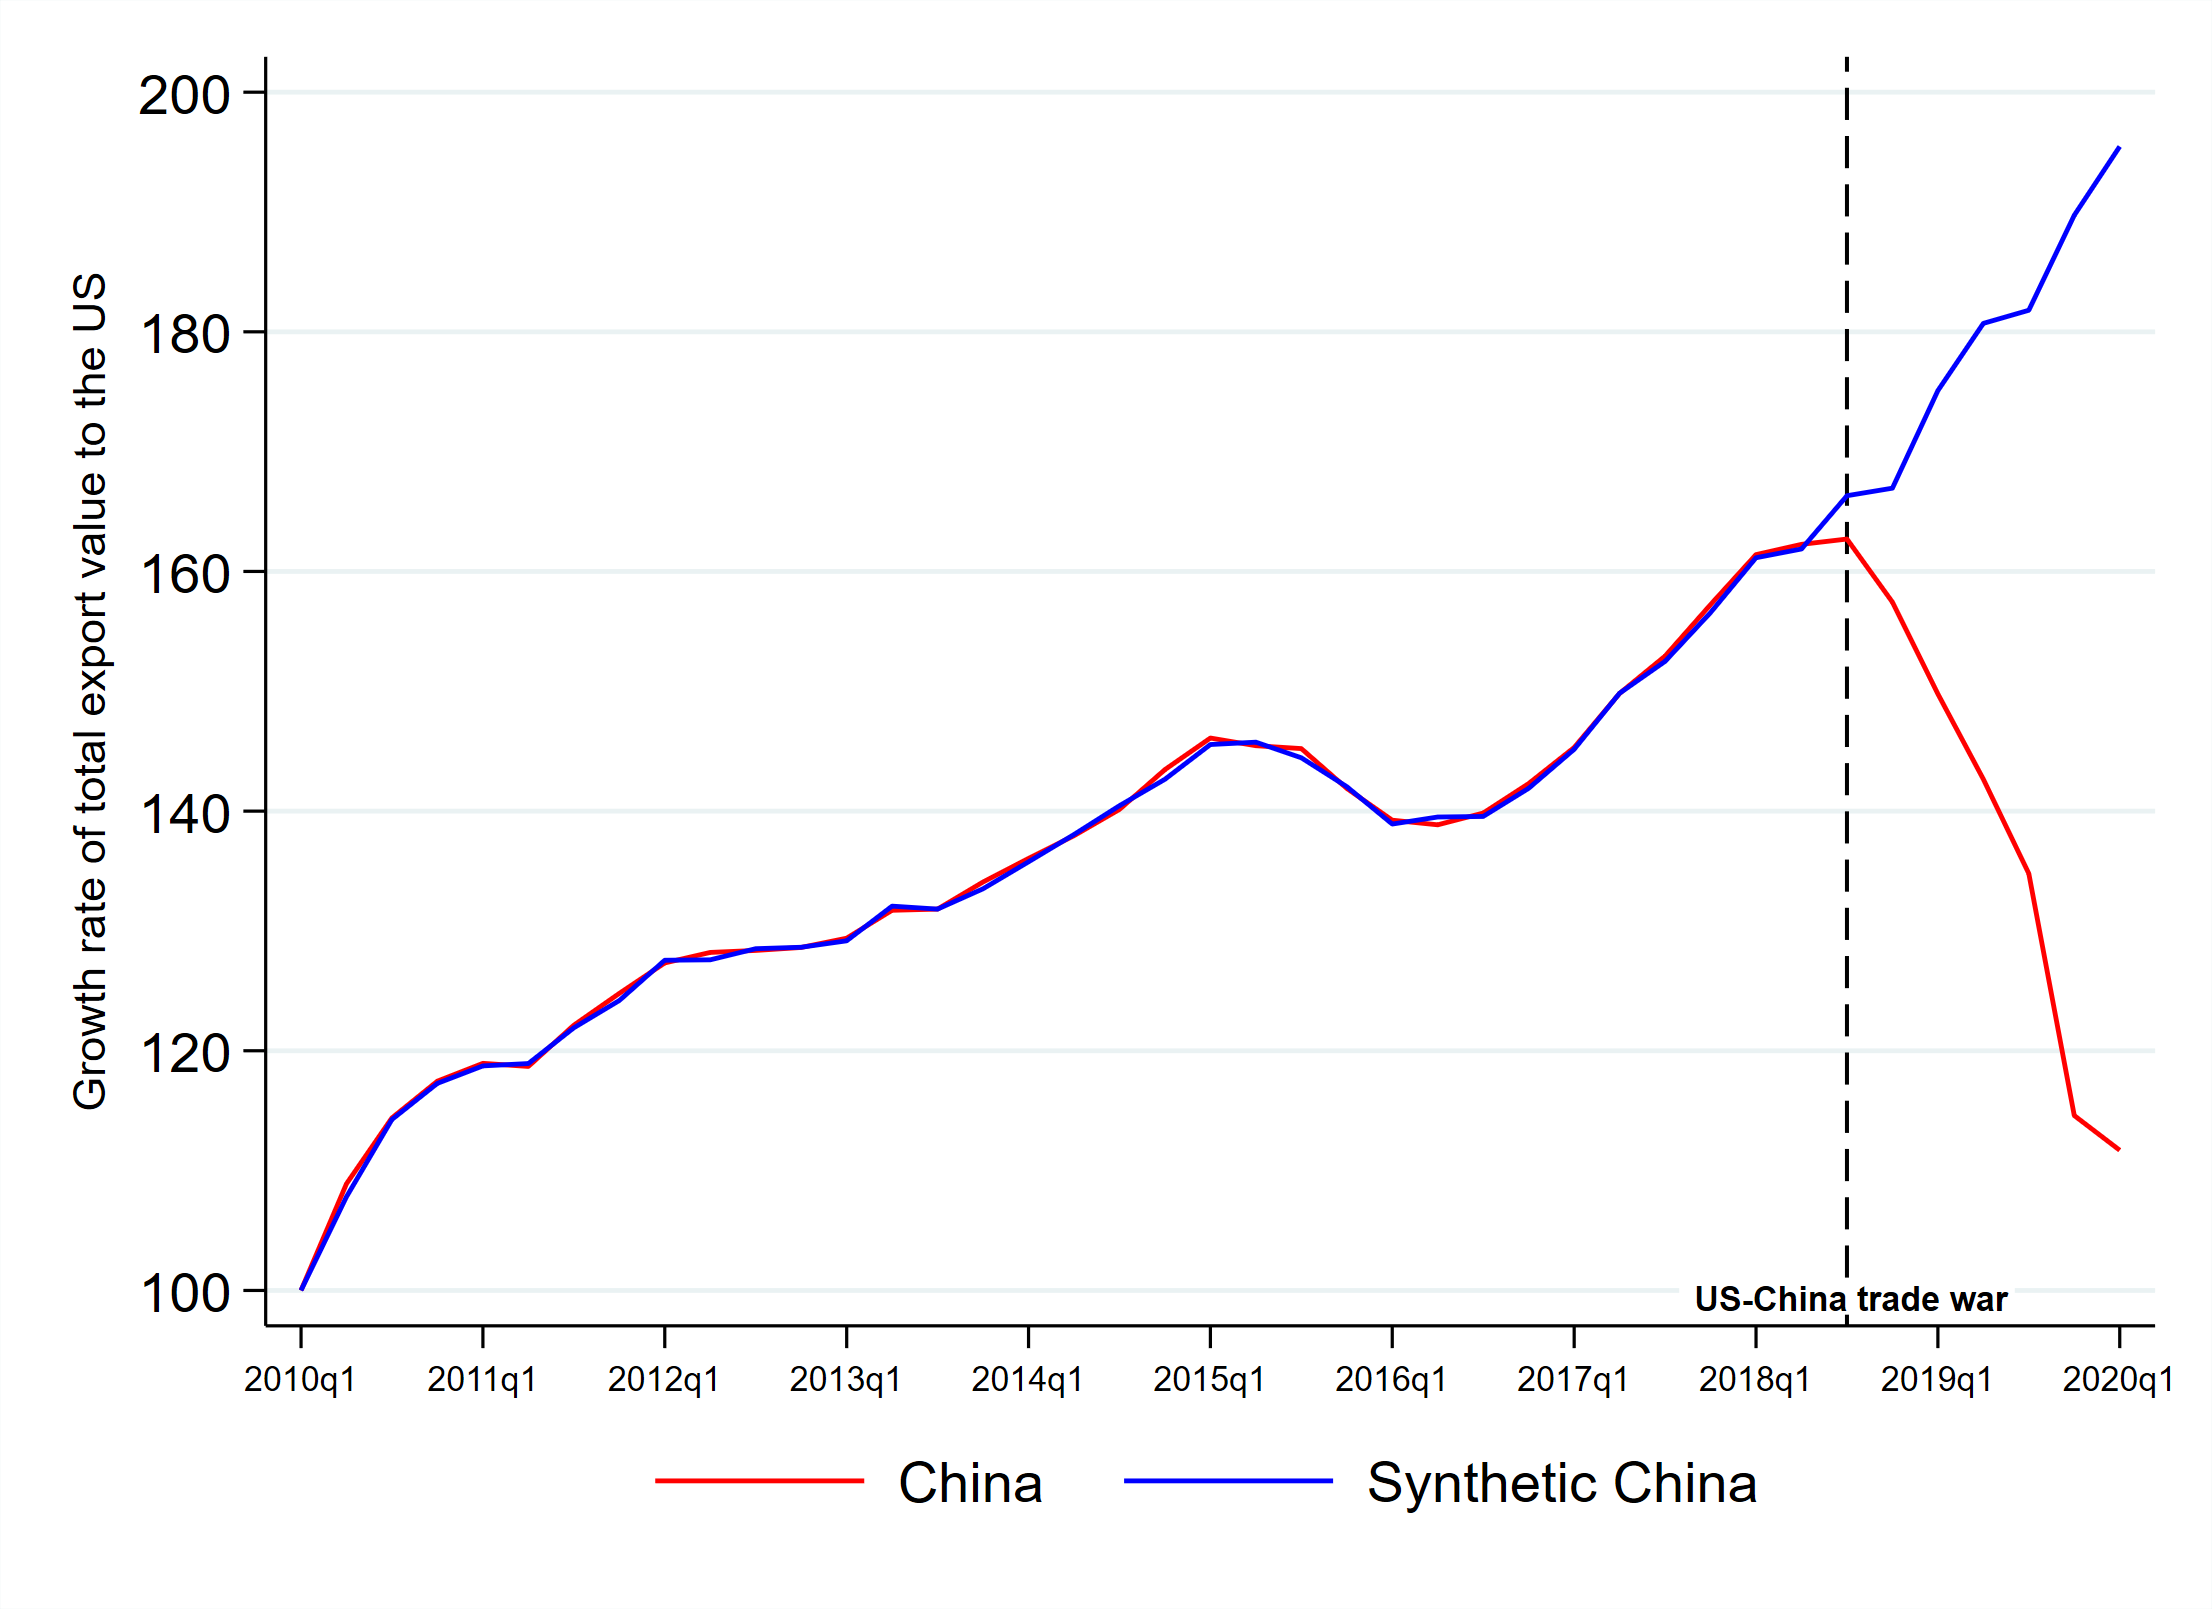
\includegraphics[width=0.8\linewidth]{figures/SCM_us_ch.png}\\
% 	\fontsize{10}{10pt}\selectfont
% 	\flushleft
% 	\emph{Notes:} Each symbol stands for one country. The total fertility rate is defined as the number of children per 1,000 women. The data year is 2020. Data source: Our World in Data \citep{owidfertilityrate,owidgdp}.
% \end{figure}
